\documentclass[a4paper,twocolumn,superscriptaddress,nofootinbib]{revtex4-2}
\usepackage[T1]{fontenc}
\usepackage[utf8]{inputenc}
\usepackage[usenames,dvipsnames,table]{xcolor}
\usepackage{amsmath,amssymb}
\usepackage{tikz}
\usepackage{pgfplots}
\usetikzlibrary{arrows}
\usetikzlibrary{calc,shapes.geometric}
\usetikzlibrary{decorations.pathmorphing}
\tikzset{
  antenna/.style={
    isosceles triangle,
    fill=black,
    minimum width=0.2cm,
    inner sep=0pt,
    shape border rotate=90
  }
}
\pgfplotsset{compat=1.18}

\begin{document}

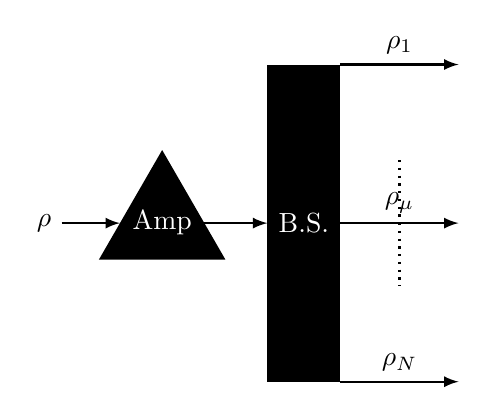
\begin{tikzpicture}[auto, thick, node distance=2.5cm, >=latex]

% Define the state rho
\node at (-2.5,0) (rho) {$\rho$};

% Add Amp - triangle
\node [draw, regular polygon, regular polygon sides=3, shape border rotate=0, fill=black, 
       minimum height=1.8cm, right of=rho, node distance=1.5cm] (amp) {};
\node[text=white] at (amp) {Amp};

% Add Beam Splitter
\node [draw, fill=black, minimum width=0.9cm, minimum height=4cm, right of=amp, node distance=1.8cm] (bs) {};
\node[text=white] at (bs) {B.S.};

% Connect the nodes
\draw [->] (rho) -- (amp.west);
\draw [->] (amp.east) -- (bs.west);

% Add output lines
\draw[->] (bs.east) -- ++(1.5,0) node[midway, above] {$\rho_\mu$};
\draw[->] (bs.north east) -- ++(1.5,0) node[midway, above] {$\rho_1$};
\draw[->] (bs.south east) -- ++(1.5,0) node[midway, above] {$\rho_N$};

% Add dotted lines
\draw[dotted] ($(bs.east) + (0.75,0.8)$) -- ($(bs.east) + (0.75,0)$);
\draw[dotted] ($(bs.east) + (0.75,0)$) -- ($(bs.east) + (0.75,-0.8)$);

\end{tikzpicture}

\end{document}